\documentclass[17pt]{extarticle}
\usepackage{tikz}
\usepackage{showexpl}
\usepackage[top=0.2in,left=0.9in]{geometry} %This geometry is page layout
\usepackage{titlesec}
\lstset
{
    language=[LaTeX]TeX,
    breaklines=true,
    basicstyle=\fontsize{14}{14}\ttfamily,
    keywordstyle=\color{blue},
    identifierstyle=\color{magenta},
}

\begin{document}
\titleformat{\section}{\normalfont\normalsize\bfseries}{\thesection}{1em}{}
\titlespacing{\section}{0pt}{0pt}{-0.3 cm}  
\section {Cartesian Coordinate System.}

\begin{LTXexample}[pos=b,preset=\centering,width=1\linewidth]
  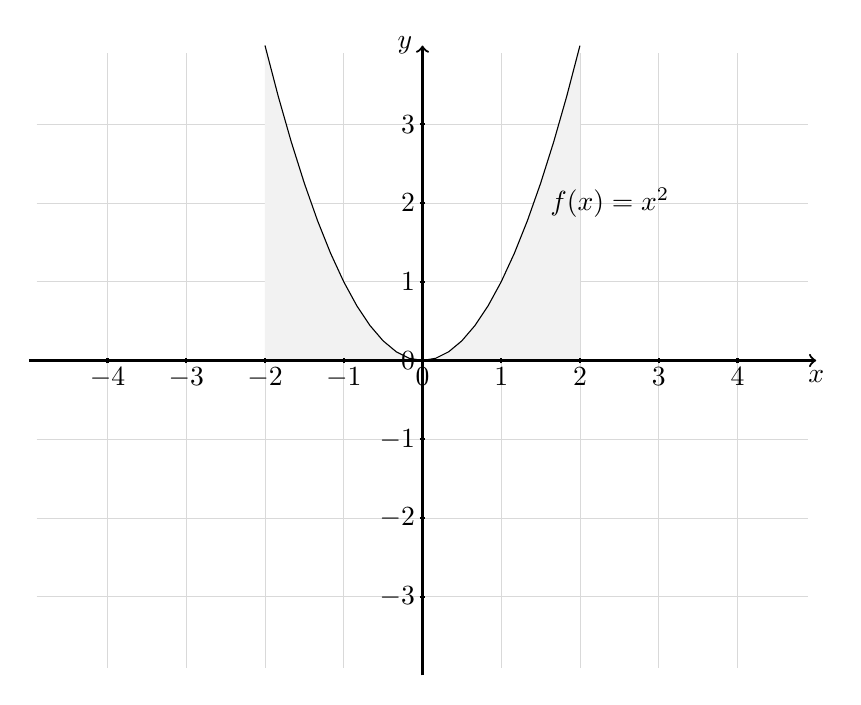
\begin{tikzpicture}
    \draw[very thin, gray!30, step=1 cm](-4.9,-3.9) grid (4.9,3.9);
    \fill [gray!10, domain=-2:2, variable=\x]
     (-2, 0) -- plot ({\x}, {\x*\x}) -- (2, 0) -- cycle;
    \draw [thick] [->] (-5,0)--(5,0) node[right, below] {$x$};
     \foreach \x in {-4,...,4}
       \draw[xshift=\x cm, thick] 
       (0pt,-1pt)--(0pt,1pt) node[below] {$\x$};
      \draw [thick] [->] (0,-4)--(0,4) node[above, left] {$y$};
     \foreach \y in {-3,...,3}
       \draw[yshift=\y cm, thick] (-1pt,0pt)--(1pt,0pt) node[left] {$\y$};

    \draw [domain=-2:2, variable=\x]
      plot ({\x}, {\x*\x}) node[right] at (1.5,2) {$f(x)=x^2$};
  \end{tikzpicture}
\end{LTXexample}

\section {red circle}
\begin{LTXexample}[pos=b,preset=\centering,width=1\linewidth]

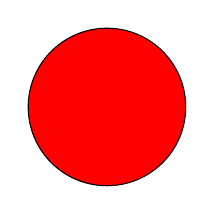
\begin{tikzpicture}
    \draw[fill=red] (0,0) circle (1);
\end{tikzpicture}

\end{LTXexample}



\section {red circle}
\begin{LTXexample}[pos=b,preset=\centering,width=1\linewidth]

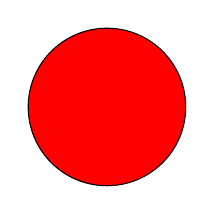
\begin{tikzpicture}
    \draw[fill=red] (0,0) circle (1);
\end{tikzpicture}

\end{LTXexample}




\end{document}